% Options for packages loaded elsewhere
\PassOptionsToPackage{unicode}{hyperref}
\PassOptionsToPackage{hyphens}{url}
\documentclass[
]{article}
\usepackage{xcolor}
\usepackage{amsmath,amssymb}
\setcounter{secnumdepth}{-\maxdimen} % remove section numbering
\usepackage{iftex}
\ifPDFTeX
  \usepackage[T1]{fontenc}
  \usepackage[utf8]{inputenc}
  \usepackage{textcomp} % provide euro and other symbols
\else % if luatex or xetex
  \usepackage{unicode-math} % this also loads fontspec
  \defaultfontfeatures{Scale=MatchLowercase}
  \defaultfontfeatures[\rmfamily]{Ligatures=TeX,Scale=1}
\fi
\usepackage{lmodern}
\ifPDFTeX\else
  % xetex/luatex font selection
\fi
% Use upquote if available, for straight quotes in verbatim environments
\IfFileExists{upquote.sty}{\usepackage{upquote}}{}
\IfFileExists{microtype.sty}{% use microtype if available
  \usepackage[]{microtype}
  \UseMicrotypeSet[protrusion]{basicmath} % disable protrusion for tt fonts
}{}
\makeatletter
\@ifundefined{KOMAClassName}{% if non-KOMA class
  \IfFileExists{parskip.sty}{%
    \usepackage{parskip}
  }{% else
    \setlength{\parindent}{0pt}
    \setlength{\parskip}{6pt plus 2pt minus 1pt}}
}{% if KOMA class
  \KOMAoptions{parskip=half}}
\makeatother
\usepackage{graphicx}
\makeatletter
\newsavebox\pandoc@box
\newcommand*\pandocbounded[1]{% scales image to fit in text height/width
  \sbox\pandoc@box{#1}%
  \Gscale@div\@tempa{\textheight}{\dimexpr\ht\pandoc@box+\dp\pandoc@box\relax}%
  \Gscale@div\@tempb{\linewidth}{\wd\pandoc@box}%
  \ifdim\@tempb\p@<\@tempa\p@\let\@tempa\@tempb\fi% select the smaller of both
  \ifdim\@tempa\p@<\p@\scalebox{\@tempa}{\usebox\pandoc@box}%
  \else\usebox{\pandoc@box}%
  \fi%
}
% Set default figure placement to htbp
\def\fps@figure{htbp}
\makeatother
\setlength{\emergencystretch}{3em} % prevent overfull lines
\providecommand{\tightlist}{%
  \setlength{\itemsep}{0pt}\setlength{\parskip}{0pt}}
\usepackage{bookmark}
\IfFileExists{xurl.sty}{\usepackage{xurl}}{} % add URL line breaks if available
\urlstyle{same}
\hypersetup{
  pdftitle={Reference-relative believability: identity{,} realism{,} and interactivity in photoreal human avatars},
  pdfauthor={D. B. Havery},
  hidelinks,
  pdfcreator={LaTeX via pandoc}}

\title{Reference-relative believability: identity, realism, and
interactivity in photoreal human avatars}
\author{D. B. Havery}
\date{}

\begin{document}
\maketitle

\emph{D. B. Havery. Working paper, v1.3 (2026-07-02).} \emph{Intended
arXiv classification: cs.HC (primary); cs.GR, cs.CV (cross-list).
Keywords: photoreal avatars, synthetic human identity, full-body
generation, talking-head synthesis, uncanny valley, face perception,
real-time conversational agents, system design.}

\subsection{Abstract}\label{abstract}

This paper comes from building avatar systems, not from trying to name a
narrow talking-head effect. The goal was a reusable engine where
character, voice, language model, and persona become a living interface:
support agent, assistant, virtual friend, presenter, virtual model, or
full-body synthetic human. Most useful identities are authored
characters, not copies of one real person. That does not make them free
of reference. A known real person has an external reference in viewer
memory. A persistent synthetic avatar has an internal reference in
canonical face, body, voice, provenance, policy, and continuity state.
Both can drift. The central claim is reference-relative believability:
avatar quality is judged against the reference available for the task,
not against pixels alone. The design consequence is an identity-contract
router. Use the high-fidelity, gated path when the output must be
indistinguishable under close human inspection. Use the low-latency path
when live presence matters more than full-body photographic proof.
Known-person likeness is one strict subcase, not the whole thesis.

\subsection{1. Introduction}\label{1-introduction}

Photoreal avatar demos have become convincing in narrow crops. A single
image and a few seconds of audio can produce a talking head that blinks,
moves its mouth, and answers questions with a face attached. Those demos
are useful, but they are also misleading. The product I kept trying to
build was not just a talking head. It was a reusable avatar engine:
character + voice + language model + persona -\textgreater{} living
interface. The same engine should support a customer-service agent, a
personal assistant, a synthetic presenter, a virtual friend, a virtual
modeling roster, and eventually full-body synthetic humans that look
like real people under high-definition inspection.

That broader target changes the problem. Most of the useful avatars are
not supposed to be a known celebrity, a public figure, or the owner of
the system. They are made-up characters. They still need to stay
themselves across sessions, outfits, poses, camera angles, lighting,
motion, and product surfaces. A modeling agency does not need a copy of
one person; it needs reusable virtual talent. An assistant does not need
to be a real employee; it needs a stable, believable presence. A content
studio does not need to impersonate someone; it needs a synthetic human
that can be reused without looking like a different person every time.

I spent several months, and close to a year if I include the earlier
digital-double work, chasing that target through the wrong abstraction.
Early systems treated support agents, assistants, presenters, full-body
avatars, and known-person likeness as variants of the same renderer
problem. They were not. Full 3D reconstruction ran into capture,
license, and fidelity walls. Blendshape bridges and procedural idle
motion looked like math. Single-image reenactment held some skin detail
but drifted head shape and expression. Mouth-only lip sync preserved
most of a real face but still failed around the mouth, teeth, and
temporal boundary. Full-body generation made the failure broader: hands,
eyes, hair, skin texture, face pixel size, garment fit, and pose
consistency all became visible. A portrait that looked acceptable became
weak once the whole body, wardrobe, camera, and motion had to survive.

The useful lesson was not simply that one method failed. It was that the
reference changed the bar. A known real person is judged against memory.
A persistent synthetic human is judged against its canonical identity
state and against the viewer\textquotesingle s category model of real
humans. A throwaway generic face is judged against a much looser bar.
Those are not the same product requirement.

This paper names that distinction reference-relative believability. The
question is not only "does the frame look real?" It is "real relative to
which reference?" For a known person, the reference is external and held
by the viewer. For a persistent synthetic character, the reference is
internal and maintained by the system. For full-body
indistinguishability, the reference is the ordinary human body under
close inspection. The system has to know which reference it is trying to
satisfy before it chooses a renderer, a latency target, a safety policy,
or an evaluation gate.

\subsection{2. The tension nobody
resolves}\label{2-the-tension-nobody-resolves}

Avatar products usually collapse three requirements into one word:
realism. In practice they are separate.

The first requirement is \textbf{human realism}: skin, hair, eyes,
hands, body proportions, clothing, camera behavior, motion, and lighting
must look like a real scene. The second is \textbf{identity continuity}:
the same character must remain the same character across outputs. The
third is \textbf{live interactivity}: the avatar must respond to
unplanned speech fast enough to feel present. A serious product cannot
treat these as one scalar score.

Full-body work makes the conflict obvious. Portrait crops hide many
failures. They keep the face large, remove hands, avoid most garment
physics, and constrain the pose. Full-body images expose the system.
Face pixels shrink below reliable identity-measurement thresholds. Hands
enter the frame. Hair, fabric, knees, shoes, posture, and body
proportions matter. A model that passes a headshot test can fail a
96-image full-body variation grid because the prompt asks for different
poses, outfits, lighting, and camera positions. That was the most
important build lesson: solving framing revealed the detail problems
that cropped demos had been hiding.

Live interaction creates a different pressure. You cannot pre-record the
answer to a question you have not been asked. A conversational avatar
has to render or drive speech-linked motion from text or audio. Today
that usually means a learned talking-head model, a portrait warper, an
audio-to-video model, or a clip library with lip-sync layered on top.
These systems can be good enough for presence. They are not
automatically good enough for high-definition full-body inspection.

The hard product problem is therefore not "can a model generate a face?"
It is deciding which bar the output must clear. A full-body virtual
model for a clothing shoot needs slower, gated, high-resolution
generation and continuity checks. A live support assistant may accept a
narrower head-and-shoulders render if it answers quickly and honestly. A
known-person likeness has an even stricter external reference because
viewers already know the source.

\subsection{3. The reference-relative
principle}\label{3-the-reference-relative-principle}

Here is the claim in plain form. A synthesized avatar is judged against
the strongest reference available for the task.

For a known real person, the reference is the viewer\textquotesingle s
stored model of that person\textquotesingle s appearance and motion. The
viewer is not evaluating a generic human image. They are comparing
against memory: jaw width, asymmetry, expression timing, eye behavior,
skin and beard texture, the way the mouth moves when thinking.
Familiar-face research already shows that known faces are processed
differently from unfamiliar faces {[}4-8{]}. Recent deepfake-detection
work makes the same point from the other direction: a 2025 systematic
review finds that viewers spot manipulations more reliably when they
already know the person\textquotesingle s face {[}16{]}. In synthesis,
that advantage becomes a stricter rejection mechanism.

For a persistent synthetic character, the reference is not viewer memory
of a real person. It is the character\textquotesingle s canonical
identity state. The system defines the face, body, age band, voice,
allowed styling range, provenance, and continuity rules. From that point
on, the character is no longer a disposable prompt result. It is a
roster identity. If the nose changes, the body proportions drift, the
face ages across shoots, or the hands and skin fail close inspection,
the output is wrong relative to the identity contract even if no real
person was copied.

For a one-off synthetic stranger, the reference is looser: the image
must belong to the category "real human" for the context. That is still
not easy. Dead eyes, waxy skin, broken fingers, incoherent lighting,
uncanny mouth motion, and temporal jitter all fail. What the one-off
stranger escapes is only the tighter comparison against a known person
or a canonical roster identity.

I use \textbf{ground-truth drift} for deviation from the applicable
reference. The source of ground truth can be external memory, internal
canonical identity, or a real-human category bar. The mistake in the
early architecture was treating made-up characters as if they had no
ground truth. That is true only before the character is committed. Once
a synthetic identity is saved and reused, it has a reference, and the
system has to defend it.

\subsection{4. The split that survived the
build}\label{4-the-split-that-survived-the-build}

The split is not "real person versus fake person." That was the wrong
shortcut. The split is between render contracts.

The \textbf{high-fidelity identity path} covers any avatar that must
survive close visual inspection: a known real person, a fixed synthetic
roster identity, a virtual model for fashion shoots, or a high-value
presenter where screenshots will be inspected. This path is allowed to
be slower. It needs canonical identity state, full-body framing,
high-resolution generation, face and body continuity checks, skin and
hand evaluation, garment realism review, provenance, and human review
when the gate is uncertain. If the identity is a real person, the path
should preserve real pixels or use extremely constrained edits. If the
identity is synthetic, synthesis is allowed, but only under continuity
gates. "Made up" does not mean "anything goes."

The \textbf{live interaction path} covers support agents, assistants,
virtual friends, and other conversational surfaces where responsiveness
is part of the product. It can use audio-driven talking heads, live
portrait animation, pre-rendered idle clips, or streaming video chunks.
Its job is presence, timing, voice, memory, and turn-taking. It still
needs safety, disclosure, and continuity, but it should not pretend to
be a full-body, high-definition proof surface unless it actually clears
that bar.

Known-person likeness sits inside the first path as the strictest
subcase. The earlier mistake was letting that subcase dominate the whole
paper. The broader product target is harder and more useful: persistent
synthetic humans that remain stable enough for modeling, assistant,
companion, and content-creation workflows while looking
indistinguishable from real people at the level users actually inspect.

\subsection{5. What the principle
predicts}\label{5-what-the-principle-predicts}

The claim is useful only if it predicts something beyond "models will
improve." Reference-relative believability predicts different failure
curves for different references.

\textbf{Familiarity gradient.} For the same synthesis pipeline and
visible artifact level, ratings should get worse as the viewer knows the
depicted real person better. The ordering should be easier for a
stranger, harder for a public figure, harder again for a close relation,
and hardest for the self.

\textbf{Canonical-continuity gradient.} Persistent synthetic characters
should become stricter over time. The first exposure may be judged
mostly against the human category. After a character is saved, reused,
named, and seen across sessions, viewers and the system both acquire a
reference. A render that would pass as a one-off stranger can fail as
"not the same avatar."

\textbf{Full-body exposure effect.} Headshot demos should overstate
quality. Moving to full-body framing should reveal failures in hands,
hair, body proportions, garment interaction, face pixel size, pose, and
lighting. If the model only passes when the face is large and the body
is hidden, it has not cleared the full avatar bar.

\textbf{Identity-swap rescue, with limits.} A renderer that fails on a
known real person may rate higher when the same motion and rendering
method are applied to a new synthetic identity. That rescue should
shrink once the synthetic identity has a canonical state and repeated
exposure.

\textbf{Latency-fidelity trade.} A low-latency path may score well for
presence and poorly for close inspection. A high-fidelity path may score
well for screenshots and poorly for live turn-taking. Treating those as
one score should produce confused product decisions.

The first study does not need a new model. Use one renderer and produce
paired clips or images across four conditions: known real person,
unfamiliar real person, newly authored synthetic identity, and
persistent synthetic identity with a prior reference set. Hold duration,
framing, voice quality, and prompt content as constant as possible.
Separately rate visible artifact severity. The key question is whether
reference condition predicts rejection after artifact severity is
controlled. If it does not, the theory is wrong or incomplete.

\subsection{6. Where this sits}\label{6-where-this-sits}

I am not proposing another renderer here. The renderer work exposed a
systems boundary.

The uncanny valley, from Mori onward {[}1{]}, gives the broad discomfort
shape when an entity becomes nearly human but not fully convincing.
Later accounts emphasize motion, category conflict, and prediction error
{[}2, 3{]}. Recent avatar studies sharpen this further: discomfort
tracks the consistency of realism cues and the interaction context
rather than raw fidelity, and the effect of appearance realism is
moderated by task and setting {[}14, 15{]}. Reference-relative
believability fits that literature, but shifts the unit of analysis. The
relevant object is not just the stimulus. It is the stimulus in relation
to a viewer and to the identity contract the system claims to preserve.

The face-perception literature explains the known-person subcase.
Familiar and self faces are processed differently from unfamiliar faces
{[}4-8{]}. That is why a near miss on a known person is rejected so
quickly. But persistent synthetic identities add another case: once the
system defines a canonical identity and repeats it across contexts, it
creates its own reference.

Talking-head and portrait-animation systems provide the live surface
{[}9-12{]}. Unified audio-to-video systems suggest that live avatar
quality will keep improving {[}13{]}. Full-body generation and
virtual-model workflows add a different surface: not just the face in
motion, but the whole human body, wardrobe, camera, and scene. Better
generators reduce drift. They do not remove the need to state which
reference the output must satisfy.

\subsection{7. The architecture this
implies}\label{7-the-architecture-this-implies}

The architecture I landed on keeps the conversational stack shared and
makes the render contract explicit.

The shared stack includes speech recognition, language model routing,
voice selection, memory, tools, transport, and policy controls. It can
serve many products. The render layer sits behind a fixed interface, but
it is not selected casually. An identity contract router decides whether
a request belongs on the high-fidelity identity path or the live
interaction path.

\pandocbounded{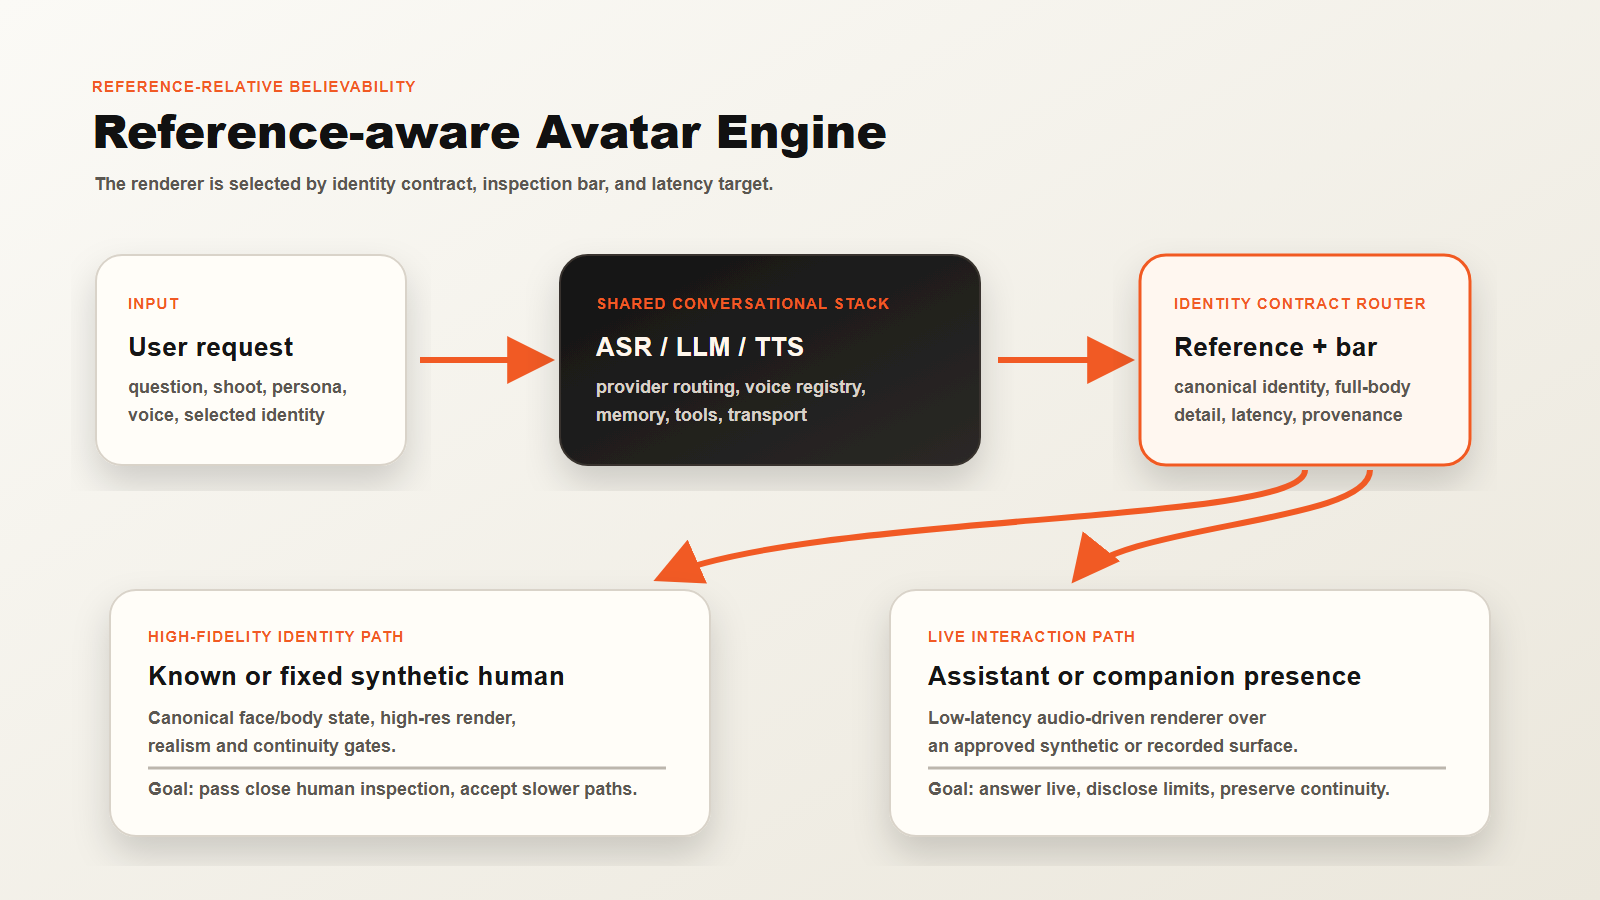
\includegraphics[keepaspectratio,alt={Reference-aware Avatar Engine architecture. Shared conversational systems feed an identity contract router; high-fidelity identities use gated render paths, while live interaction surfaces use low-latency render paths.}]{assets/two-tier-avatar-engine.png}}

\emph{Figure 1. Reference-aware Avatar Engine architecture. The
conversational stack is shared. The renderer is selected by identity
contract, inspection bar, latency target, and provenance requirement.}

The high-fidelity identity path treats a character as more than a face
prompt. It carries canonical face state, body state, allowed styling
range, identity references, evaluation thresholds, provenance, and
safety policy. Outputs are gated for realism and continuity: face, skin,
hands, body, garment interaction, camera coherence, and identity drift.
This is the path for virtual modeling, high-value presenters,
known-person likeness, and any artifact expected to survive zoomed-in
review by a human viewer.

The live interaction path treats presence and timing as first-class
requirements. It can use a narrower crop, a talking-head renderer,
pre-rendered idle clips, a browser stream, or a real-time provider. It
still uses the same character registry and policy layer, but it should
be labeled as a live interaction surface rather than a proof of
full-body indistinguishability.

In my current implementation, the boundary is concrete. The private
Avatar Engine repository defines character registries, a renderer
protocol, and user-choice registries for character, voice, and language
model. A local loop connects speech recognition, an Ollama language
model, Piper voice synthesis, and a Ditto talking-head renderer.
TensorRT made the Ditto path fast enough for the real-time tier. A
resident worker keeps the renderer warm, and a streaming path can render
answer chunks as they complete. In parallel, separate high-fidelity
identity-planning work defines the other side: identity creation, roster
state, full-body variation grids, realism gates, continuity services,
provenance, and human review.

The unfinished parts are also part of the result. Full-duplex barge-in,
browser transport, idle behavior, latency polish, full-body video, and
garment-level production remain engineering work. The theory does not
make those easy. It says they should not be hidden behind one generic
"photoreal" label.

\subsection{8. Limitations and safety}\label{8-limitations-and-safety}

I have not measured the full curve yet. I have a build history,
falsifiable predictions, and a working architecture boundary, not a
completed human-subjects study. The curve may vary by culture, screen
size, task, exposure duration, artifact type, and whether the user is
judging utility, comfort, trust, or visual truth.

The reference can also move. A synthetic assistant that starts as a new
character may become familiar after repeated use. A virtual model roster
may start with an authored canonical state and then tighten as clients
approve specific shoots. A model upgrade may improve general realism
while breaking continuity. The architecture has to treat identity state
as durable product data, not as prompt history.

This is not an argument for irresponsible synthetic humans. It is the
opposite. Synthetic identities should be created with consent-safe
source rules, age safeguards, similarity checks, disclosure, provenance
(for example, signed content credentials {[}17{]}), and audit logs.
Known-person likeness needs explicit consent and stricter renderer
constraints. Persistent synthetic identity needs continuity gates and
policy controls because realism increases the practical risk of misuse.
A system that cannot say where an identity came from, what it is allowed
to do, and which renderer may touch it is not ready.

\subsection{9. Conclusion}\label{9-conclusion}

The first version of this argument was too narrow. It made the
known-person case the center. The bigger and more useful thesis is that
photoreal avatars are reference-relative systems. A known person is
judged against memory. A persistent synthetic human is judged against
canonical identity state and the real-human category. A live assistant
is judged against presence, timing, disclosure, and continuity. A
full-body virtual model is judged against high-definition human detail:
face, skin, eyes, hair, hands, body, garment, camera, and motion.

The practical rule is simple. Do not ask one renderer to satisfy every
reference. Route by identity contract. Put full-body, close-inspection
avatars on a gated high-fidelity path. Put conversational presence on a
live interaction path. Treat made-up characters as real product objects
once they are saved. That is not a retreat from the original
avatar-engine vision. It is the version that survived contact with the
work.

\subsection{References}\label{references}

{[}1{]} M. Mori, "The uncanny valley," \emph{Energy}, vol. 7, no. 4, pp.
33-35, 1970. Trans. K. F. MacDorman and N. Kageki, \emph{IEEE Robotics
\& Automation Magazine}, vol. 19, no. 2, pp. 98-100, 2012.

{[}2{]} A. P. Saygin, T. Chaminade, H. Ishiguro, J. Driver, and C.
Frith, "The thing that should not be: predictive coding and the uncanny
valley in perceiving human and humanoid robot actions," \emph{Social
Cognitive and Affective Neuroscience}, vol. 7, no. 4, pp. 413-422, 2012.

{[}3{]} R. K. Moore, "A Bayesian explanation of the
\textquotesingle uncanny valley\textquotesingle{} effect and related
psychological phenomena," \emph{Scientific Reports}, vol. 2, art. 864,
2012.

{[}4{]} V. Bruce and A. Young, "Understanding face recognition,"
\emph{British Journal of Psychology}, vol. 77, no. 3, pp. 305-327, 1986.

{[}5{]} R. A. Johnston and A. J. Edmonds, "Familiar and unfamiliar face
recognition: a review," \emph{Memory}, vol. 17, no. 5, pp. 577-596,
2009.

{[}6{]} A. M. Burton, S. Wilson, M. Cowan, and V. Bruce, "Face
recognition in poor-quality video: evidence from security surveillance,"
\emph{Psychological Science}, vol. 10, no. 3, pp. 243-248, 1999.

{[}7{]} P. J. B. Hancock, V. Bruce, and A. M. Burton, "Recognition of
unfamiliar faces," \emph{Trends in Cognitive Sciences}, vol. 4, no. 9,
pp. 330-337, 2000.

{[}8{]} F. Tong and K. Nakayama, "Robust representations for faces:
evidence from visual search," \emph{Journal of Experimental Psychology:
Human Perception and Performance}, vol. 25, no. 4, pp. 1016-1035, 1999.

{[}9{]} K. R. Prajwal, R. Mukhopadhyay, V. P. Namboodiri, and C. V.
Jawahar, "A lip sync expert is all you need for speech to lip generation
in the wild" (Wav2Lip), in \emph{Proc. ACM Int. Conf. Multimedia (MM)},
2020, pp. 484-492.

{[}10{]} J. Guo et al., "LivePortrait: efficient portrait animation with
stitching and retargeting control," arXiv:2407.03168, 2024.

{[}11{]} T. Li, R. Zheng, M. Yang, J. Chen, and M. Yang, "Ditto:
motion-space diffusion for controllable realtime talking head
synthesis," arXiv:2411.19509, 2024 (ACM MM 2025).

{[}12{]} S. Xu et al., "VASA-1: lifelike audio-driven talking faces
generated in real time," in \emph{Advances in Neural Information
Processing Systems (NeurIPS)}, 2024. arXiv:2404.10667.

{[}13{]} Wan Team, Alibaba Group, "Wan-Streamer v0.1: end-to-end
real-time interactive foundation models," arXiv:2606.25041, 2026.

{[}14{]} T. D. Do, R. P. McMahan, and P. J. Wisniewski, "A new uncanny
valley? The effects of speech fidelity and human listener gender on
social perceptions of a virtual-human speaker," in \emph{Proc. CHI Conf.
Human Factors in Computing Systems (CHI \textquotesingle22)}, 2022.

{[}15{]} Z. Tao, Y. Liu, J. Qiu, and S. Li, "Impact of virtual avatar
appearance realism on perceptual interaction experience: a network
meta-analysis," \emph{Frontiers in Psychology}, vol. 16, art. 1624975,
2025.

{[}16{]} K. Somoray, D. Miller, and M. Holmes, "Human performance in
deepfake detection: a systematic review," \emph{Human Behavior and
Emerging Technologies}, 2025, doi:10.1155/hbe2/1833228.

{[}17{]} Coalition for Content Provenance and Authenticity, "C2PA
technical specification (Content Credentials)," version 2.2, 2025.
{[}Online{]}. Available: \url{https://c2pa.org/specifications/}

\end{document}
